\documentclass[noauthor,nooutcomes,hints,handout,12pt]{ximera}

\graphicspath{  
{./}
{./whoAreYou/}
{./drawingWithTheTurtle/}
{./bisectionMethod/}
{./circles/}
{./anglesAndRightTriangles/}
{./lawOfSines/}
{./lawOfCosines/}
{./plotter/}
{./staircases/}
{./pitch/}
{./qualityControl/}
{./symmetry/}
{./nGonBlock/}
}


%% page layout
\usepackage[cm,headings]{fullpage}
\raggedright
\setlength\headheight{13.6pt}


%% fonts
\usepackage{euler}

\usepackage{FiraMono}
\renewcommand\familydefault{\ttdefault} 
\usepackage[defaultmathsizes]{mathastext}
\usepackage[htt]{hyphenat}

\usepackage[T1]{fontenc}
\usepackage[scaled=1]{FiraSans}

%\usepackage{wedn}
\usepackage{pbsi} %% Answer font


\usepackage{cancel} %% strike through in pitch/pitch.tex


%% \usepackage{ulem} %% 
%% \renewcommand{\ULthickness}{2pt}% changes underline thickness

\tikzset{>=stealth}

\usepackage{adjustbox}

\setcounter{titlenumber}{-1}

%% journal style
\makeatletter
\newcommand\journalstyle{%
  \def\activitystyle{activity-chapter}
  \def\maketitle{%
    \addtocounter{titlenumber}{1}%
                {\flushleft\small\sffamily\bfseries\@pretitle\par\vspace{-1.5em}}%
                {\flushleft\LARGE\sffamily\bfseries\thetitlenumber\hspace{1em}\@title \par }%
                {\vskip .6em\noindent\textit\theabstract\setcounter{question}{0}\setcounter{sectiontitlenumber}{0}}%
                    \par\vspace{2em}
                    \phantomsection\addcontentsline{toc}{section}{\thetitlenumber\hspace{1em}\textbf{\@title}}%
                     }}
\makeatother



%% thm like environments
\let\question\relax
\let\endquestion\relax

\newtheoremstyle{QuestionStyle}{\topsep}{\topsep}%%% space between body and thm
		{}                      %%% Thm body font
		{}                              %%% Indent amount (empty = no indent)
		{\bfseries}            %%% Thm head font
		{)}                              %%% Punctuation after thm head
		{ }                           %%% Space after thm head
		{\thmnumber{#2}\thmnote{ \bfseries(#3)}}%%% Thm head spec
\theoremstyle{QuestionStyle}
\newtheorem{question}{}



\let\freeResponse\relax
\let\endfreeResponse\relax

%% \newtheoremstyle{ResponseStyle}{\topsep}{\topsep}%%% space between body and thm
%% 		{\wedn\bfseries}                      %%% Thm body font
%% 		{}                              %%% Indent amount (empty = no indent)
%% 		{\wedn\bfseries}            %%% Thm head font
%% 		{}                              %%% Punctuation after thm head
%% 		{3ex}                           %%% Space after thm head
%% 		{\underline{\underline{\thmname{#1}}}}%%% Thm head spec
%% \theoremstyle{ResponseStyle}

\usepackage[tikz]{mdframed}
\mdfdefinestyle{ResponseStyle}{leftmargin=1cm,linecolor=black,roundcorner=5pt,
, font=\bsifamily,}%font=\wedn\bfseries\upshape,}


\ifhandout
\NewEnviron{freeResponse}{}
\else
%\newtheorem{freeResponse}{Response:}
\newenvironment{freeResponse}{\begin{mdframed}[style=ResponseStyle]}{\end{mdframed}}
\fi



%% attempting to automate outcomes.

%% \newwrite\outcomefile
%%   \immediate\openout\outcomefile=\jobname.oc
%% \renewcommand{\outcome}[1]{\edef\theoutcomes{\theoutcomes #1~}%
%% \immediate\write\outcomefile{\unexpanded{\outcome}{#1}}}

%% \newcommand{\outcomelist}{\begin{itemize}\theoutcomes\end{itemize}}

%% \NewEnviron{listOutcomes}{\small\sffamily
%% After answering the following questions, students should be able to:
%% \begin{itemize}
%% \BODY
%% \end{itemize}
%% }
\usepackage[tikz]{mdframed}
\mdfdefinestyle{OutcomeStyle}{leftmargin=2cm,rightmargin=2cm,linecolor=black,roundcorner=5pt,
, font=\small\sffamily,}%font=\wedn\bfseries\upshape,}
\newenvironment{listOutcomes}{\begin{mdframed}[style=OutcomeStyle]After answering the following questions, students should be able to:\begin{itemize}}{\end{itemize}\end{mdframed}}



%% my commands

\newcommand{\snap}{{\bfseries\itshape\textsf{Snap!}}}
\newcommand{\flavor}{\link[\snap]{https://snap.berkeley.edu/}}
\newcommand{\mooculus}{\textsf{\textbf{MOOC}\textnormal{\textsf{ULUS}}}}


\usepackage{tkz-euclide}
\tikzstyle geometryDiagrams=[rounded corners=.5pt,ultra thick,color=black]
\colorlet{penColor}{black} % Color of a curve in a plot



\ifhandout\newcommand{\mynewpage}{\newpage}\else\newcommand{\mynewpage}{}\fi


\title{Sine and cosine}
\author{Bart Snapp}

\begin{document}
\begin{abstract}
  Sine and cosine encode information about similar right triangles.
\end{abstract}
\maketitle

\begin{listOutcomes}
\item Recall the basic definitions of sine and cosine.
\item View sine and cosine as encoding information about similar right
  triangles.
\item Explain basic facts about sine and cosine based on their
  definitions.
\item Extend the basic definition of sine to include obtuse angles. 
\end{listOutcomes}



\begin{definition}
 Two triangles are said to be \textbf{similar} if their corresponding angles all have the same measure.  In this case, one triangle is a scaled version of the other triangle.
\end{definition}


\mynewpage


\begin{question}
  Consider the following right triangle:
  \begin{center}
      \begin{tikzpicture}[geometryDiagrams]
        \coordinate (A) at (0,0);
        \coordinate (B) at (0,3);
        \coordinate (C) at (7,0);
        \tkzDrawSegment (A,B)
        \tkzDrawSegment (A,C)
        \tkzDrawSegment (C,B)
        \tkzLabelSegment[left](A,B){$a$}
        \tkzLabelSegment[below](A,C){$b$}
        \tkzLabelSegment[above right](B,C){$c$}  

        \tkzMarkRightAngle[thin](C,A,B)
        %\tkzLabelAngle[pos=1.2](C,A,B){$?$}

        \tkzMarkAngle[size=0.8cm,thin,mark=](A,B,C)
        \tkzLabelAngle[pos=.5](A,B,C){$\beta$}

        \tkzMarkAngle[mark=,size=1.2cm,thin](B,C,A)
        \tkzLabelAngle[pos=.9](B,C,A){$\alpha$}
      \end{tikzpicture}
    \end{center}
  \begin{enumerate}
  \item Either look up or remember the definitions of \textbf{sine}
    and \textbf{cosine} of both $\alpha$ and $\beta$ in terms of this
    right triangle's hypotenuse, opposite leg, and adjacent leg. State them here as you would like them stated to you.  
    \item Explain why $\sin(\alpha) =
    \cos(90^\circ-\alpha)$ and why $\cos(\alpha) =
    \sin(90^\circ-\alpha)$.
\end{enumerate}
\end{question}
\mynewpage



\begin{question}    
We can extend the definition of sine to \textbf{any} triangle if we
interpret it as follows: Given any triangle, find a height $h$
perpendicular to a side. Then use the right triangle to
$\sin(\theta)$.

\begin{enumerate}
 \item Use similar triangles to explain why 
      \[
      \frac{h}{c} = \frac{h'}{b}
      \]
     in the following diagrams. The side lengths and angles of the triangle with solid lines are the same in both diagrams.
     

 
      \begin{center}
        \begin{tikzpicture}[geometryDiagrams]
          \coordinate (A) at (0,0);
          \coordinate (B) at (5,2);
          \coordinate (C) at (7,0);
         \draw(0,0)--(5,2)--(7,0)--(0,0);
	 \draw (0,0)--(5,2) node [midway,yshift=.3cm] {$c$};
         \draw [decorate,decoration={brace,amplitude=10pt,mirror},thin](0,0)--(7,0) node [midway,yshift=-.6cm] {$b$};
          \draw (7,0)--(5,2) node [midway,yshift=.3cm] {$a$};
          \tkzMarkAngle[size=1.5cm,thin,mark=](C,A,B)
          \tkzLabelAngle[pos=1.2](C,A,B){$\theta$}

          \tkzDefPointsBy[projection=onto A--C](B){D}.
          
          \tkzMarkRightAngle[thin](B,D,C)
          \tkzDrawSegment[dashed](B,D)
          \tkzLabelSegment[left](D,B){$h$}  
        \end{tikzpicture}
      \end{center}
      
       \begin{center}
        \begin{tikzpicture}[geometryDiagrams]
          \coordinate (A) at (0,0);
          \coordinate (B) at (5,2);
          \coordinate (C) at (7,0);
	\draw(0,0)--(5,2)--(7,0)--(0,0);
	\draw (0,0)--(5,2) node [midway,yshift=.3cm] {$c$};
         \draw (0,0)--(7,0) node [midway,yshift=-.3cm] {$b$};
          \draw (7,0)--(5,2) node [midway,yshift=.3cm] {$a$};
          \tkzMarkAngle[size=1.5cm,thin,mark=](C,A,B)
          \tkzMarkAngle[size=1.5cm,thin,mark=](C,A,B)
          \tkzLabelAngle[pos=1.2](C,A,B){$\theta$}

          
          \tkzMarkAngle[size=1.5cm,thin,mark=](C,A,B)
          \tkzLabelAngle[pos=1.2](C,A,B){$\theta$}
          
          \tkzDefPointsBy[projection=onto A--B](C){D}
          \tkzDrawSegment[dashed](C,D)
          \tkzMarkRightAngle[thin](B,D,C)
          \tkzLabelSegment[right](D,C){$h'$}
          \tkzDrawSegment[dashed](D,B)
        \end{tikzpicture}
      \end{center}
      
     \item       
       Explain why in this definition of sine, \textbf{it doesn't matter which
         height we choose, the value of $\boldsymbol{\sin(\theta)}$ will be the same.}

     \item Confirm that $\frac{h}{c} = \frac{h'}{b}$ in the diagrams
       above by \textbf{measuring with a ruler,} and hence directly computing
       $\sin(\theta)$.
        \end{enumerate}
\end{question}

\mynewpage

\begin{question}
  Explain how to compute sine of an obtuse angle.
\end{question}

\end{document}
%  \begin{freeResponse}
%    \begin{enumerate}
%    \item Given a right triangle,
%      \begin{center}
%        \begin{tikzpicture}[geometryDiagrams]
%          \coordinate (A) at (0,0);
%          \coordinate (B) at (0,3);
%          \coordinate (C) at (7,0);
%          \tkzDrawSegment (A,B)
%          \tkzDrawSegment (A,C)
%          \tkzDrawSegment (C,B)
%          \tkzLabelSegment[left](A,B){$a$}
%          \tkzLabelSegment[below](A,C){$b$}
%          \tkzLabelSegment[above right](B,C){$c$}  
%          
%          \tkzMarkRightAngle[thin](C,A,B)
%          %\tkzLabelAngle[pos=1.2](C,A,B){$?$}
%          
%          \tkzMarkAngle[size=0.8cm,thin,mark=](A,B,C)
%          \tkzLabelAngle[pos=.5](A,B,C){$\beta$}
%          
%          \tkzMarkAngle[mark=,size=1.2cm,thin](B,C,A)
%          \tkzLabelAngle[pos=.9](B,C,A){$\alpha$}
%        \end{tikzpicture}
%      \end{center}
%      if we are working with the angle of measure $\alpha$,
%      \[
%      \sin(\alpha) = \frac{\text{opposite}}{\text{hypotenuse}} = \frac{a}{c},
%      \]
%      and
%    \[
%    \cos(\alpha) = \frac{\text{adjacent}}{\text{hypotenuse}} = \frac{b}{c}.
%    \]
%    If we are working with the angle of measure $\beta$,
%    \[
%    \sin(\beta) = \frac{\text{opposite}}{\text{hypotenuse}} = \frac{b}{c},
%    \]
%    and
%    \[
%    \cos(\beta) = \frac{\text{adjacent}}{\text{hypotenuse}} = \frac{a}{c}.
%    \]
%    From this we immediately see that
%    \[
%    \sin(\alpha) = \cos(\beta),
%    \]
%    and since $\beta = 180-90-\alpha$, we see
%    \[
%    \sin(\alpha) = \cos(90-\alpha).
%    \]
%    In an entirely similar way, we have
%    \[
%    \cos(\alpha) = \sin(90-\alpha).
%    \]
%
%  \item Note that the triangle with hypotenuse $c$ and ``short'' leg
%    $h$ is a scaled copy of the triangle with hypotenuse $b$ and
%    ``short'' leg $h'$.
%    Thus
%    \[
%    c = s\cdot b\qquad{and}h = s\cdot h'
%    \]
%    Now we see
%    \[
%    \sin(\theta) = \frac{h}{c} = \frac{s\cdot b}{s\cdot h'} = \frac{b}{h'}.
%    \]
%    \item To see $\sin(180-\theta)=\sin(\theta)$ check this out:
%      \begin{center}
%      \begin{tikzpicture}[geometryDiagrams]
%        \coordinate (A) at (0,0);
%        \coordinate (B) at (4.33,0);
%        \coordinate (C) at (-4.33,2.5);
%        \coordinate (D) at (-4.33,0);
%        
%        \coordinate (AA) at (0,0);
%        \coordinate (BB) at (4.33,0);
%        \coordinate (CC) at (4.33,2.5);
%
%        \tkzDrawSegment[red,dashed](C,D)
%        \tkzDrawSegment[red,line width=2pt](A,B)
%        \tkzDrawSegment[red,line width=2pt](A,C)
%        \tkzDrawSegment[red,line width=2pt](C,B)
%        \tkzLabelSegment[red,below left](A,C){$c$}
%
%        \tkzDrawSegment[red,dashed](A,D)
%        
%        \tkzMarkRightAngle[red,thin](A,D,C)
%        \tkzMarkAngle[red,mark=,size=1.4cm,thin](BB,AA,C)
%        \tkzLabelAngle[red,pos=.7](BB,A,C){$180-\theta$};
%
%        \tkzDrawSegment[blue,line width=2pt](AA,BB)
%        \tkzDrawSegment[blue,line width=2pt](AA,CC)
%        \tkzDrawSegment[blue,line width=2pt](CC,BB)
%        \tkzLabelSegment[blue,above left](AA,CC){$c$}
%
%        \tkzLabelSegment[blue,right](BB,CC){$h$}
%        \tkzLabelSegment[red,left](C,D){$h$}
%        
%        \tkzMarkRightAngle[blue,thin](AA,BB,CC)
%        \tkzMarkAngle[blue,mark=,size=1.2cm,thin](BB,AA,CC)
%        \tkzLabelAngle[blue,pos=.9](BB,AA,CC){$\theta$};
%      \end{tikzpicture}
%      \end{center}
%      And so we see
%      \[
%      \sin(180-\theta)=\frac{h}{c}=\sin(\theta).
%      \]
%    \end{enumerate}
%    \end{freeResponse}
%\end{question}
%\mynewpage
%
%\begin{question}
%  Now imagine a right triangle with a hypotenuse of length $1$. 
%  \begin{enumerate}
%  \item For a given nonright angle of the triangle, call it $\theta$,
%    EXPLAIN why one leg of the triangle has length $\cos(\theta)$ and
%    the other has length $\sin(\theta)$.  Use words, pictures, and so
%    on, as needed/helpful in your explanation.
%  \item EXPLAIN why
%    \[
%    \cos^2(\theta) + \sin^2(\theta) = 1.
%    \]
%  \item Use your work above to EXPLAIN why
%    \[
%    (x,y) = (\sin(\theta),\cos(\theta))
%    \]
%    will always lie on a unit circle centered at the origin for any
%    angle $\theta$.
%  \end{enumerate}
%  \begin{freeResponse}
%    \begin{enumerate}
%    \item Given a right triangle
%    \begin{center}
%      \begin{tikzpicture}[geometryDiagrams]
%        \coordinate (A) at (0,0);
%        \coordinate (B) at (0,3);
%        \coordinate (C) at (7,0);
%        \tkzDrawSegment (A,B)
%        \tkzDrawSegment (A,C)
%        \tkzDrawSegment (C,B)
%        \tkzLabelSegment[left](A,B){$a$}
%        \tkzLabelSegment[below](A,C){$b$}
%        \tkzLabelSegment[above right](B,C){$1$}  
%
%        \tkzMarkRightAngle[thin](C,A,B)
%        %\tkzLabelAngle[pos=1.2](C,A,B){$?$}
%
%        %\tkzMarkAngle[size=0.8cm,thin,mark=](A,B,C)
%        %\tkzLabelAngle[pos=.5](A,B,C){$\beta$}
%
%        \tkzMarkAngle[mark=,size=1.2cm,thin](B,C,A)
%        \tkzLabelAngle[pos=.9](B,C,A){$\theta$}
%      \end{tikzpicture}
%    \end{center}
%    We see
%    \[
%    \sin(\theta) = \frac{a}{1} = a\qquad \text{and}\qquad \cos(\theta) = \frac{b}{1} = b.
%    \]
%  \item With the same right triangle above, we also see via the Pythagorean theorem:
%    \[
%    \cos^2(\theta) + \sin^2(\theta) = 1.
%    \]
%  \item Since
%    \[
%    x^2+y^2=1
%    \]
%    is the set of points making a unit circle and
%    \[
%    \sin^2(\theta) + \cos^2(\theta) = 1
%    \]
%    we see that $x=\sin(\theta)$ and $y=\cos(\theta)$ will always be
%    on the circle.
%    \end{enumerate}
%  \end{freeResponse}
%\end{question}
%\mynewpage
%
%
%\begin{question}
%  Let's think about our previous work a little more.
%  \begin{enumerate}
%  \item Consider the following \snap\ block \raisebox{-.4\height}{
\includegraphics{circleBlank.png}}. Here is the script for that block:
%    \begin{center}
%      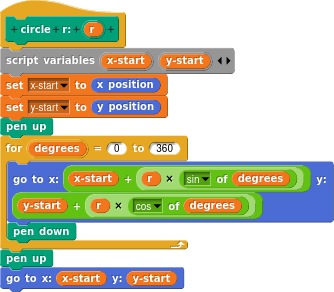
\includegraphics{circleScript.png}
%    \end{center}
%    EXPLAIN how the script works, block-by-block as you would like to
%    have it explained to you. Use words, pictures, and so on, as
%    needed/helpful in your explanation.
%  \item Some folks like to plot circles with:
%    \[
%    (x,y) = (\cos(\theta),\sin(\theta)) \qquad\text{others with}\qquad  (x,y) = (\sin(\theta),\cos(\theta))
%    \]
%    How does the command \raisebox{-.4\height}{
\includegraphics{circleBlank.png}} change if you change how it plots circles?
%  \item Find REAL WORLD circumstances where it might be better to use $(x,y) = (\sin(\theta),\cos(\theta))$. EXPLAIN your reasoning.
%  \item Find REAL WORLD circumstances where it might be better to use $(x,y) = (\cos(\theta),\sin(\theta))$. EXPLAIN your reasoning.
%  
%  \end{enumerate}
%  \begin{freeResponse}
%    \begin{enumerate}
%    \item Here we go:
%      \begin{enumerate}
%      \item The user tells us the radius $r$.
%      \item We have variables \texttt{x-start} and \texttt{y-start}
%        and we set them to the current position of the turtle.
%      \item Next we pick up the pen and move to the first point on the circle.
%      \item Now for each degree, we move to another point on the circle, $x= \texttt{x-start} + \sin(\theta)$. $y= \texttt{y-start} + \cos(\theta)$. 
%      \item Finally, we pick up the pen and return to where we started.
%      \end{enumerate}
%    \item As written, the command starts drawing the circle at the top
%      and travels in a clockwise direction. If we swap sine and
%      cosine, then it will start at the right and travel in a
%      counterclockwise direction.
%    \item So it would be better to use $(x,y) =
%      (\sin(\theta),\cos(\theta))$ when modeling a clock, as a clock starts at the top and travels clockwise.
%    \item It would be better to use $(x,y) =
%      (\cos(\theta),\sin(\theta))$ when modeling latitude, as the
%      equator is at zero degrees, then we travel up to the pole at
%      $90$ degrees.
%    \end{enumerate}
%  \end{freeResponse}
%\end{question}
%
%
%\end{document}
